\documentclass[aspectratio=169]{beamer}

\usepackage[utf8]{inputenc}
\usepackage[spanish]{babel}
\usepackage{graphicx}
\usepackage{booktabs}
\usepackage{ragged2e}
\usepackage{minted}
\usepackage{xcolor}
\usepackage{tikz}
\usepackage{algorithm}
\usepackage{algorithmic}
\usepackage{minted}
\usepackage{listings}
\usepackage{tikz}
\usetikzlibrary{arrows.meta,positioning,fit,shapes.symbols}
\usetikzlibrary{arrows,shapes}
\definecolor{LightGray}{gray}{0.975}
\definecolor{links}{HTML}{2A1B81}
\hypersetup{colorlinks,linkcolor=,urlcolor=blue}

\usefonttheme{serif}

\title[Backup / Restore]{Database Administration}
\subtitle{Lecture 07: Backup and Restore.}
\author{Valeja \& Gonzales.}
\date{\today}

% Remove navigation symbols...
\setbeamertemplate{navigation symbols}{}

\defbeamertemplate*{footline}{shadow theme}{
    \leavevmode
    \hbox{
        \begin{beamercolorbox}[
                wd =        0.33\paperwidth,
                ht =        2.5ex,
                dp =        1.125ex,
                leftskip =  0.3cm plus1fil,
                rightskip = 0.3cm
            ]{author in head/foot}
            \flushleft DBA
        \end{beamercolorbox}
        \begin{beamercolorbox}[
                wd =        0.33\paperwidth,
                ht =        2.5ex,
                dp =        1.125ex,
                leftskip =  0.3cm plus1fil,
                rightskip = 0.3cm
            ]{author in head/foot}
            \insertshorttitle
        \end{beamercolorbox}
        \begin{beamercolorbox}[
                wd =        0.33\paperwidth,
                ht =        2.5ex,
                dp =        1.125ex,
                leftskip =  0.3cm plus1fil,
                rightskip = 0.3cm
            ]{title in head/foot}
            \hfill \insertframenumber\,/\,\inserttotalframenumber%
        \end{beamercolorbox}
    }
}

\AtBeginSection[]
{
     \begin{frame}<beamer>
     \frametitle{Plan}
     \tableofcontents[currentsection]
     \end{frame}
}

\newcommand{\toRight}[1]{
    \begin{FlushRight}
        {\tiny #1}
    \end{FlushRight}
} % Align to right

\begin{document}

\frame{\titlepage}

\begin{frame}{Database Administration: Backup and Restore.}
    \centering
    
\includegraphics[width=0.35\textwidth]{figures/book_cover}\\
    \vspace{2mm}
    {
        \scriptsize
        Content has been extracted from \textit{PostgreSQL for Jobseekers (Chapter 7)}, by Sonia Valeja and David Gonzales, 2023.  Visit \url{https://bpbonline.com/products/postgresql-for-jobseekers}.\\
    }
\end{frame}

\section{Introduction}

\begin{frame}{Introduction}
    \begin{itemize}
        \item Regular backups are crucial for database administration.
        \item Backups enable recovery from accidental changes.
        \item PostgreSQL provides multiple backup and restore tools.
    \end{itemize}
\end{frame}

\section{Types of Backups}

\begin{frame}{Types of Backups}
    \begin{itemize}
        \item \textbf{Physical Backup}: Copies entire data directory.
        \item \textbf{Logical Backup}: Exports data in human-readable format.
    \end{itemize}
\end{frame}

\begin{frame}{Types of Backups}
    \centering
    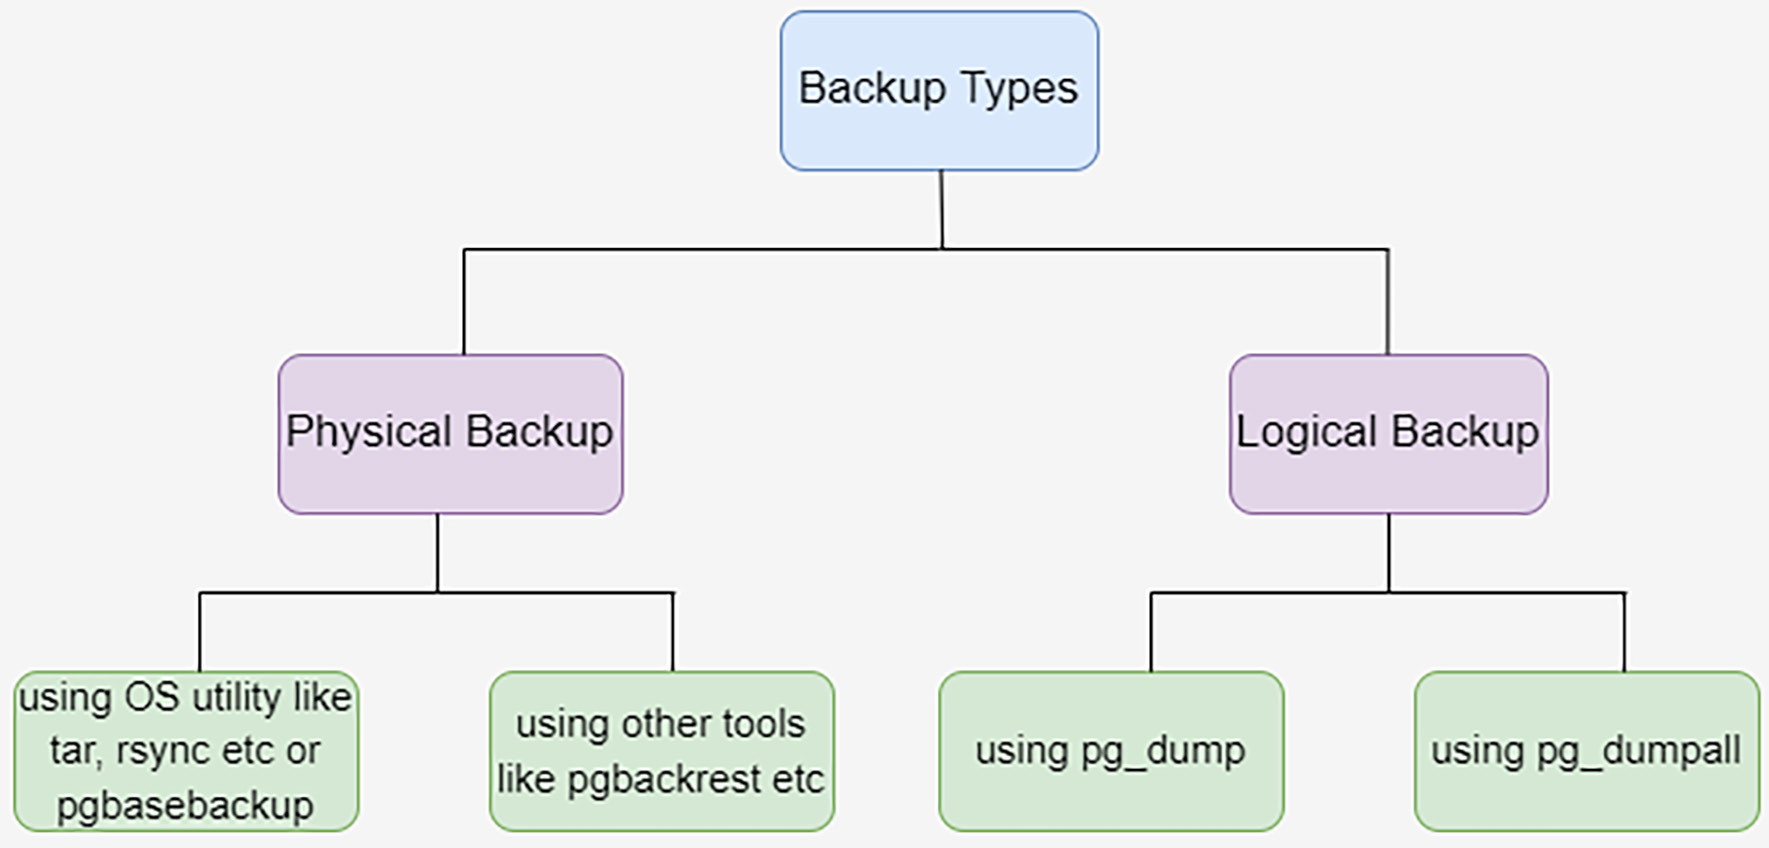
\includegraphics[width=\textwidth]{figures/backup_types}
\end{frame}

\subsection{Physical}

\begin{frame}{Physical Backup}
    \begin{itemize}
        \item Uses filesystem-level copying.
        \item Steps:
        \begin{enumerate}
            \item Create a checkpoint.
            \item Copy data directory (e.g., using \texttt{tar} or \texttt{rsync}).
            \item Stop backup process.
        \end{enumerate}
        \item Example tool: \texttt{pg\_basebackup}.
    \end{itemize}
\end{frame}

\begin{frame}{pg\_basebackup}
    \centering
    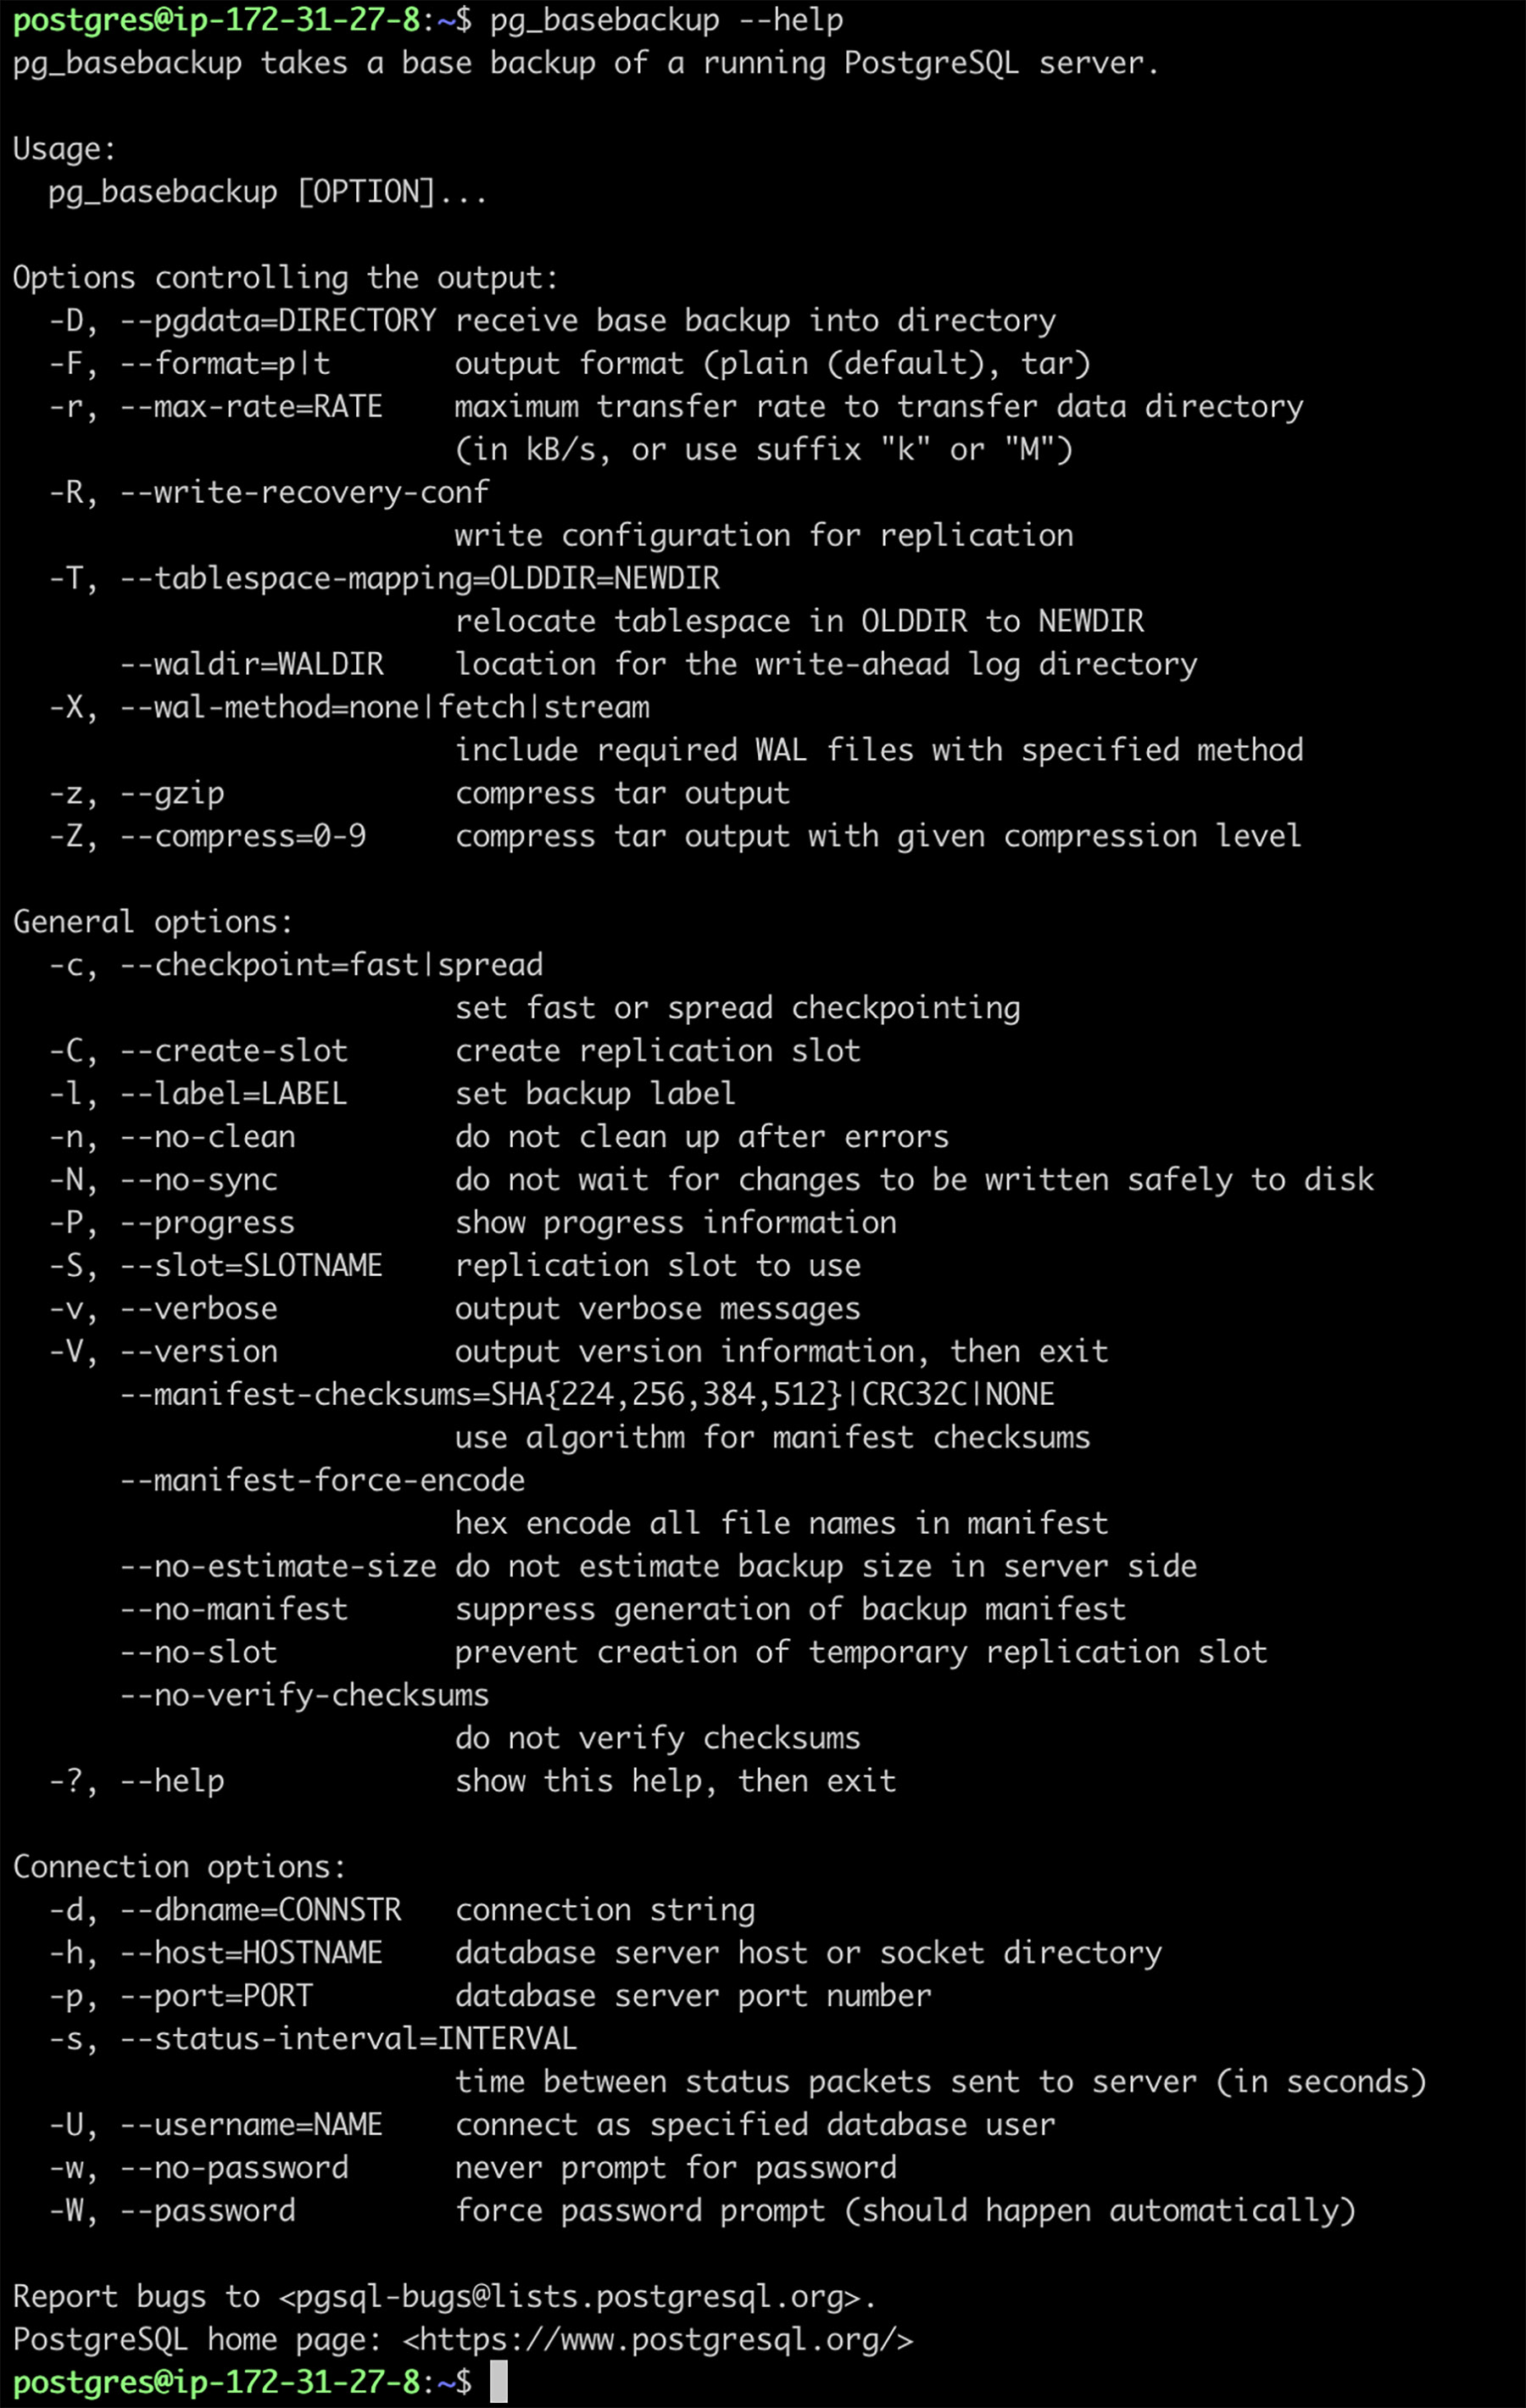
\includegraphics[width=\textwidth, trim={0cm 68cm 0cm 0cm}, clip]{figures/pg_basebackup}
\end{frame}

\begin{frame}[fragile]{Point in Time Recovery (PITR) / Archival}
    \textbf{PITR} by enabling \textbf{archiving}, this allows restoring the database to a specific time frame, provided that WAL\footnote{Write-Ahead Logging}/archives are restored until that point.

    \vspace{0.3cm}
    \textbf{Steps:}
    \begin{itemize}
        \item Enable archiving in \texttt{postgresql.conf}.
        \item Configure the following parameters:
    \end{itemize}

    \vspace{0.3cm}
    \textbf{Configuration Example:}
    \begin{verbatim}
archive_mode = on
archive_command = 'test ! -f /mnt/server/archivedir/%f && \
    cp %p /mnt/server/archivedir/%f' # Linux
archive_command = 'copy "%p" "C:\\server\\archivedir\\%f"' # Windows
    \end{verbatim}
    \vspace{-5mm}
    \toRight{\tiny We will see in the restore section how to recover a database to a specific time frame.}
\end{frame}

\begin{frame}{Pros and Cons of Physical Backup}
    \textbf{Pros:}
    \begin{itemize}
        \item Contains a full filesystem-level backup of the data directory.
        \item Includes configuration files such as \texttt{postgresql.conf}, \texttt{pg\_hba.conf}, etc.
        \item Simple process: copy the data directory and custom tablespaces to the destination server and start PostgreSQL.
    \end{itemize}

    \vspace{0.3cm}
    \textbf{Cons:}
    \begin{itemize}
        \item Only cluster-level backups are possible (no single database or table backup).
        \item Consistency of the backup is difficult to guarantee.
        \item Backup/restore speed depends heavily on server hardware and network speed (for remote copies).
    \end{itemize}
\end{frame}

\subsection{Logical}

\begin{frame}{Logical Backup}
    \begin{itemize}
        \item Exports data in SQL format.
        \item Allows individual table or database backups.
        \item Example tools:
        \begin{itemize}
            \item \texttt{pg\_dump} for single database.
            \item \texttt{pg\_dumpall} for full cluster backup.
        \end{itemize}
    \end{itemize}
\end{frame}

\begin{frame}{pg\_dump}
    \centering
    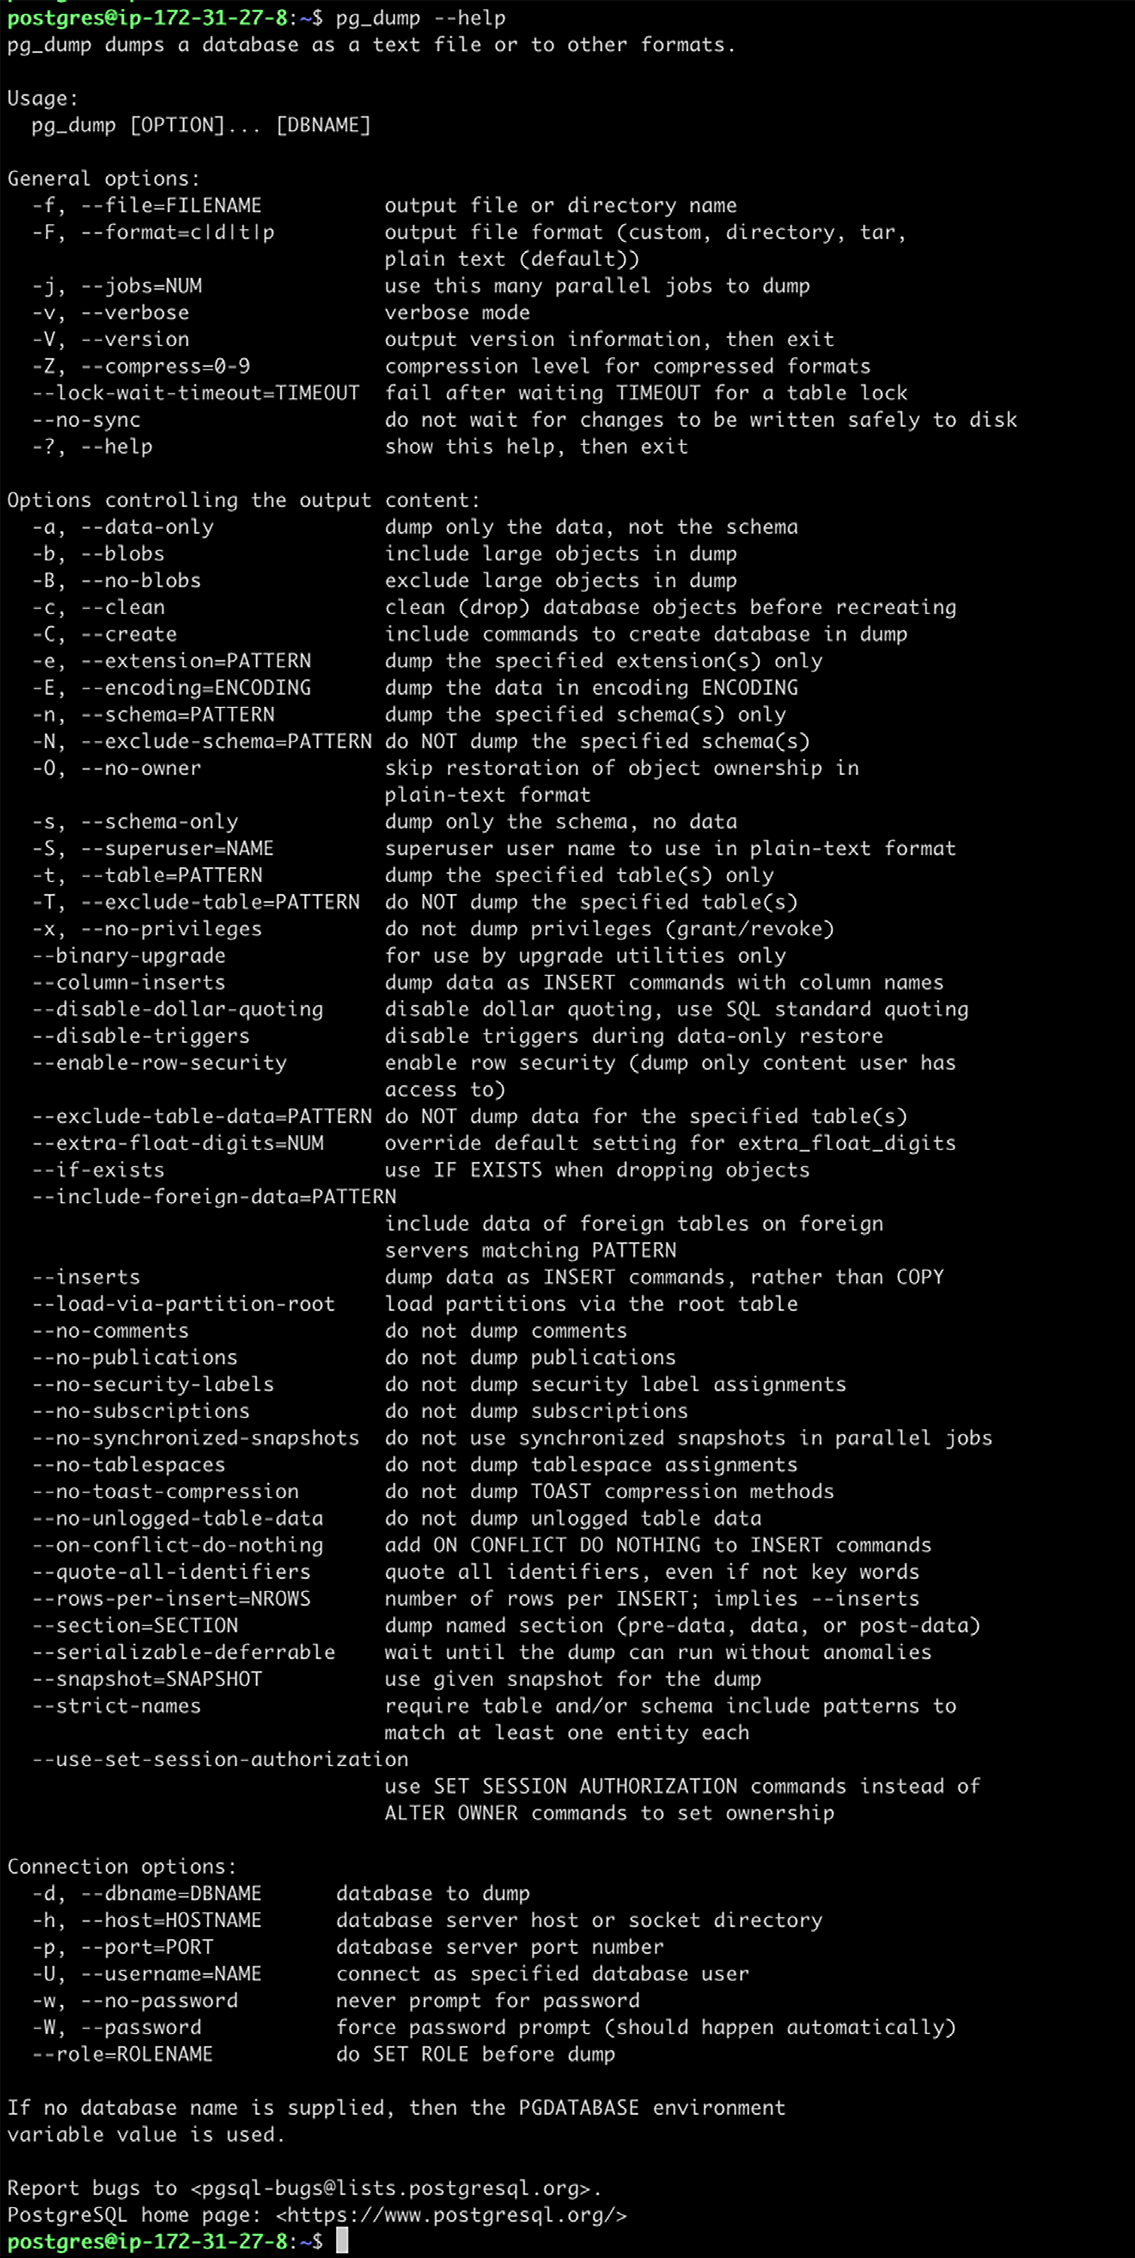
\includegraphics[width=\textwidth, trim={0cm 57.5cm 0cm 0.2cm}, clip]{figures/pg_dump}
\end{frame}

\begin{frame}{Pros and Cons of Logical Backup}
    \textbf{Pros:}
    \begin{itemize}
        \item Can back up specific parts of the database (not just the entire cluster).
        \item Simple and human-readable format.
        \item Backups are stored as plain text/SQL files, making them portable across different operating systems.
        \item Faster than physical backup when only a single DB object is required.
    \end{itemize}

    \vspace{0.3cm}
    \textbf{Cons:}
    \begin{itemize}
        \item Configuration files are not included (must be backed up separately).
        \item Point-in-Time Recovery (PITR) is not supported.
    \end{itemize}
\end{frame}

\section{Types of Restore}

\begin{frame}{Types of Restore}
    \centering
    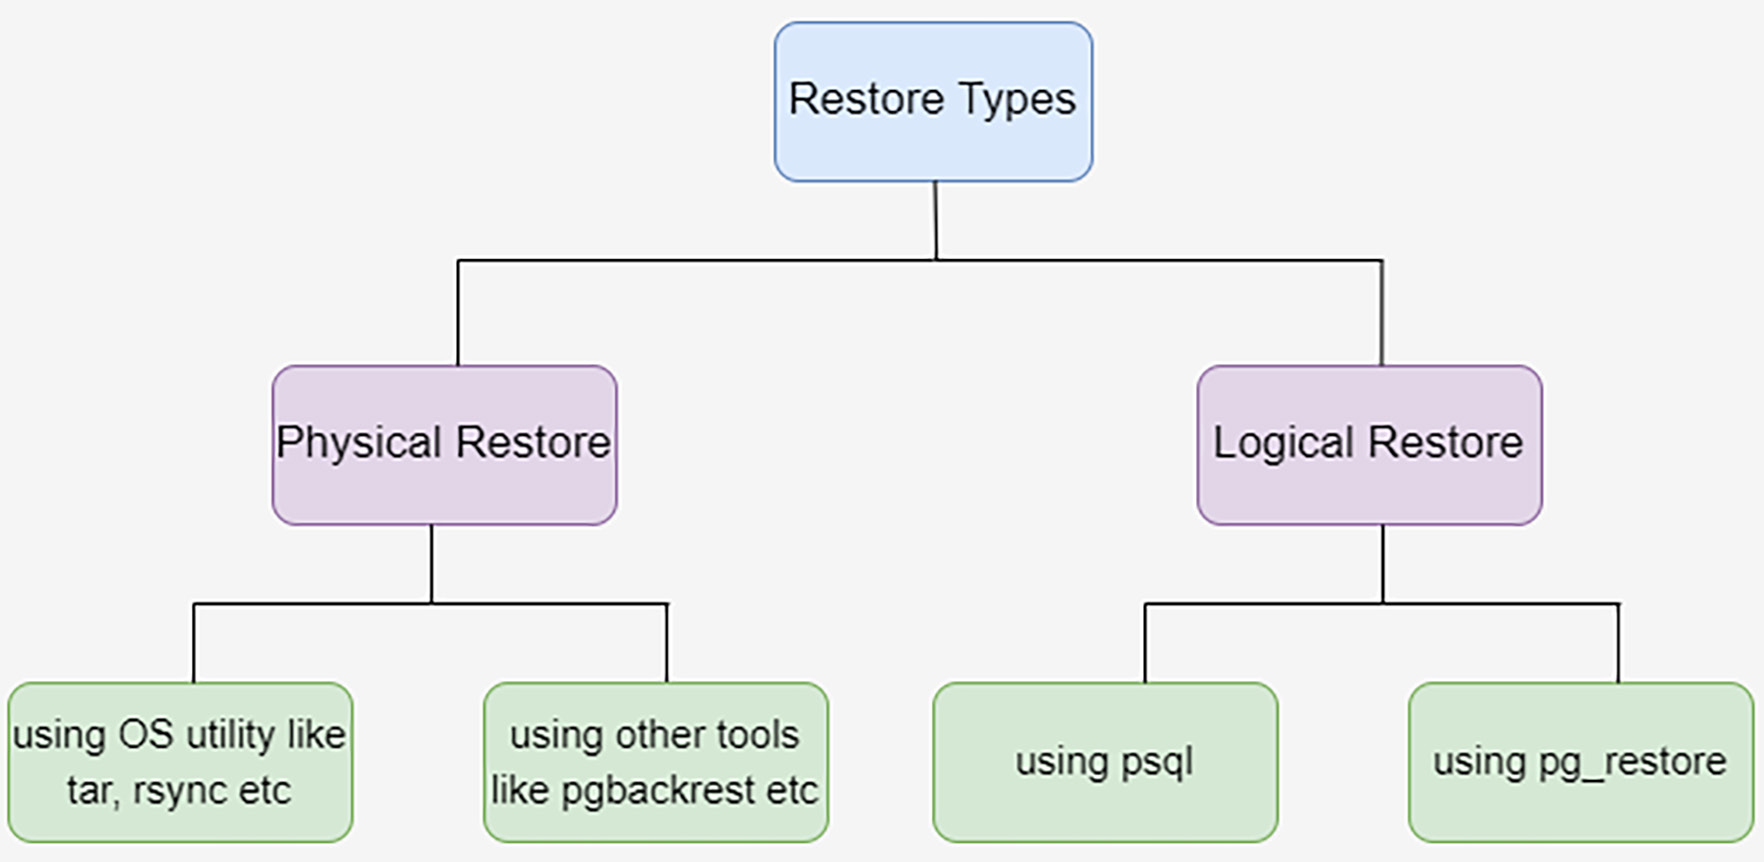
\includegraphics[width=\textwidth]{figures/restore_types}
\end{frame}

\begin{frame}{Restore Methods}
    \begin{itemize}
        \item \texttt{psql}: Restores backups in plain SQL format.
        \item \texttt{pg\_restore}: Restores backups from compressed/custom format.
    \end{itemize}
\end{frame}

\begin{frame}{pg\_restore}
    \centering
    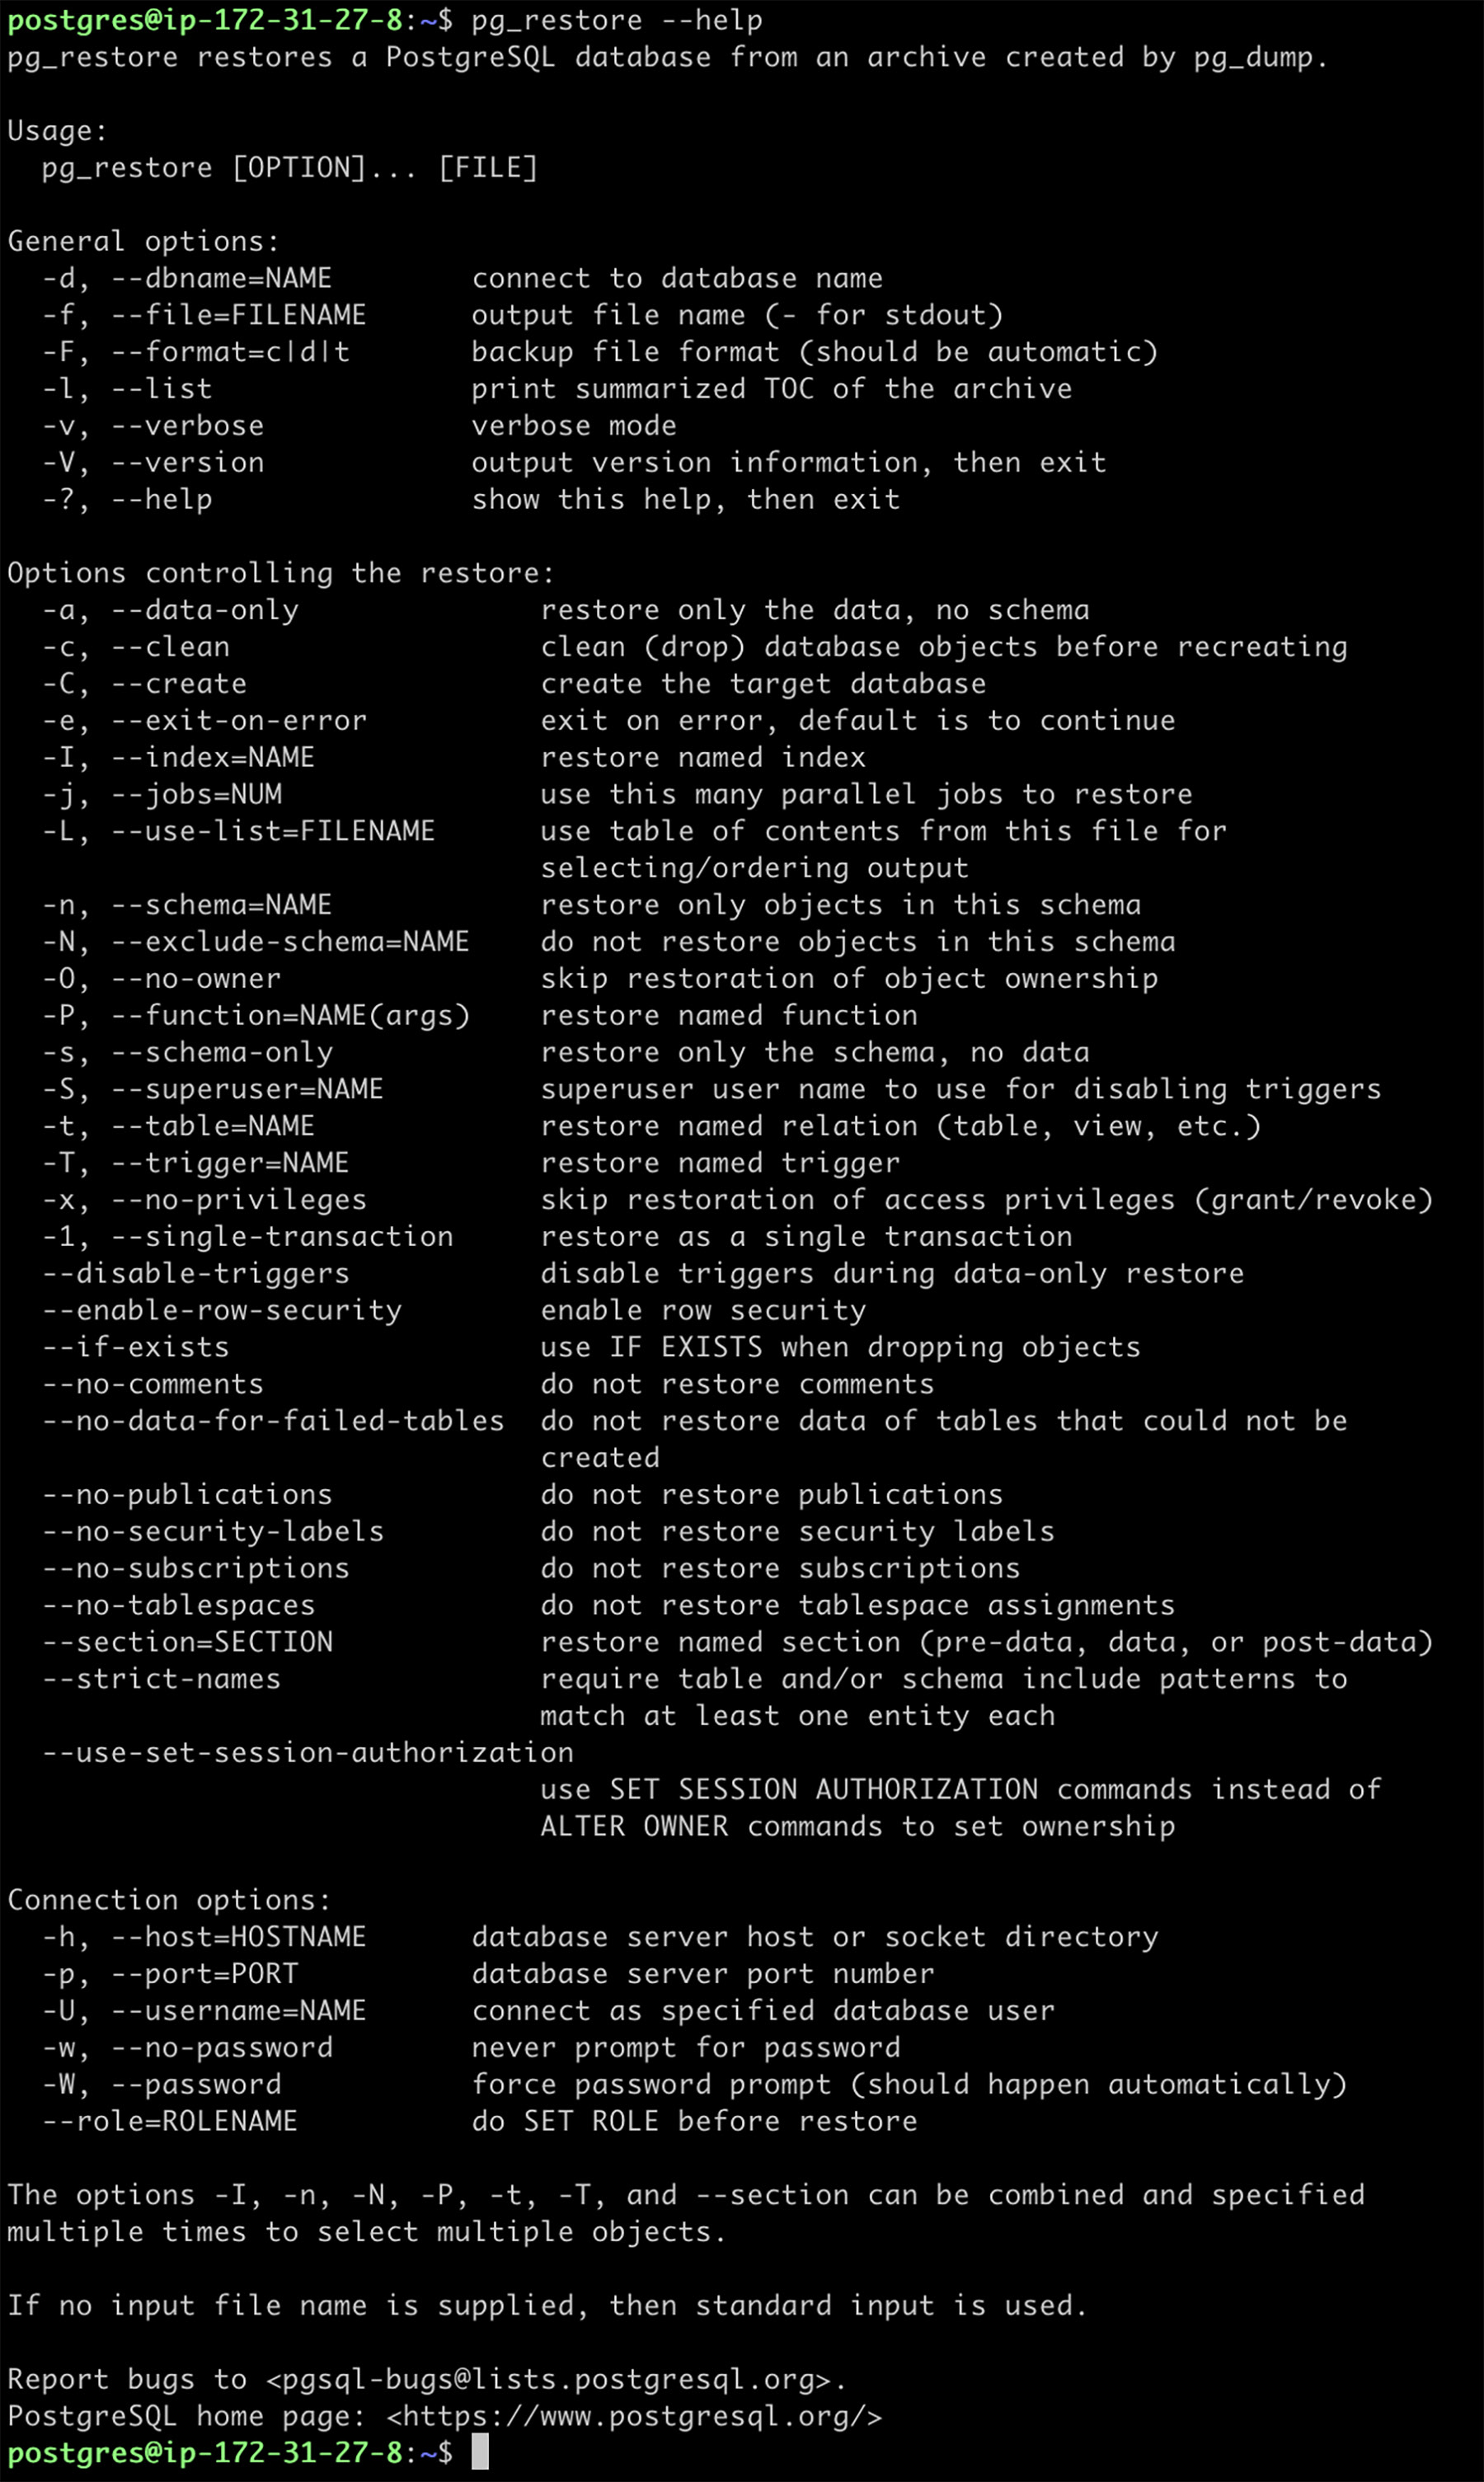
\includegraphics[width=\textwidth, trim={0cm 73cm 0cm 0cm}, clip]{figures/pg_restore}
\end{frame}

\begin{frame}{Logical Backup and Restore example}
    \centering
    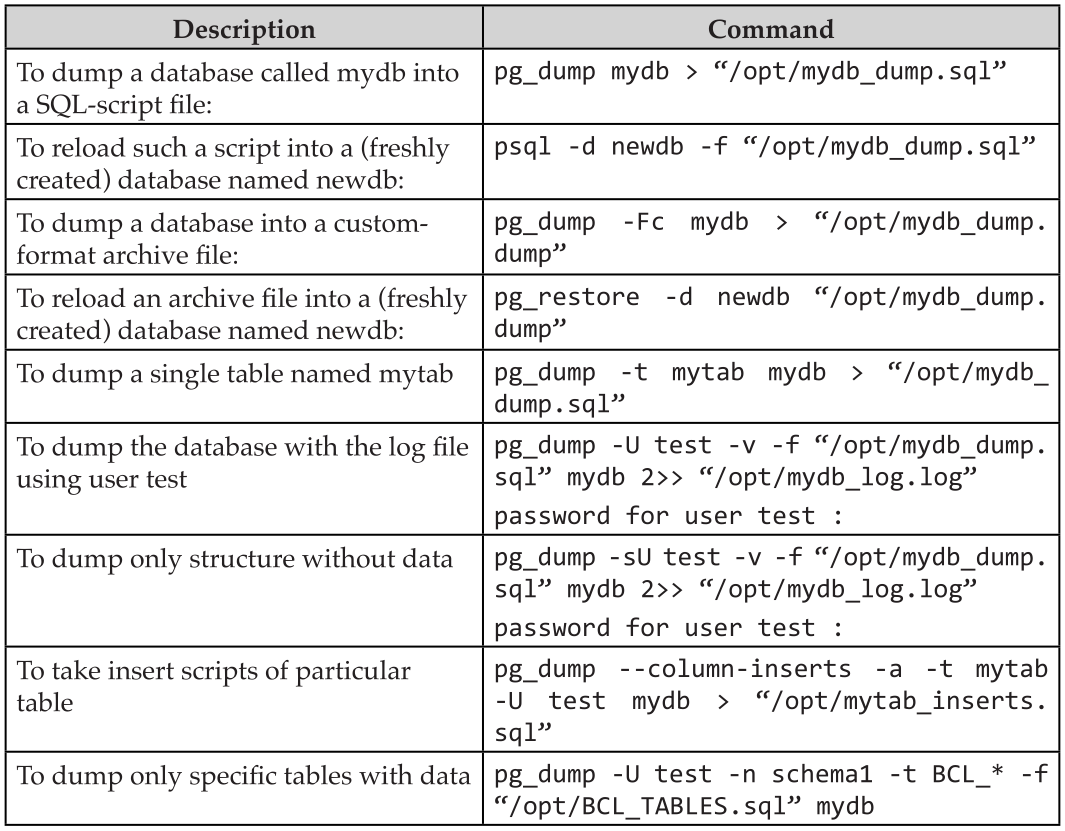
\includegraphics[width=0.7\textwidth]{figures/table}
\end{frame}

\begin{frame}{Useful Backup and Restore Tools}
    \textbf{Community-developed tools:}
    \begin{itemize}
        \item Support full, incremental, and differential backups.
        \item Provide backup compression and checksum.
        \item Allow multiple repositories: on-premise or cloud.
        \item Enable parallelism for faster operations.
        \item Maintain a backup catalog.
        \item Offer alerting and notification features.
    \end{itemize}

    \textit{We will next review some of the most popular open-source tools, their options, and how to perform a backup and restore.}
\end{frame}

\section{Advanced Backup Tools}

\begin{frame}{BiT}
    \centering
    \href{https://youtu.be/ur57IunS9To?si=-SAIS_yF9kMLX_mg}{
        
\includegraphics[width=0.5\textwidth]{figures/BiT}
    }
\end{frame}

\begin{frame}{BiT}
    \centering
    \href{https://backintime.readthedocs.io/en/latest/}{
        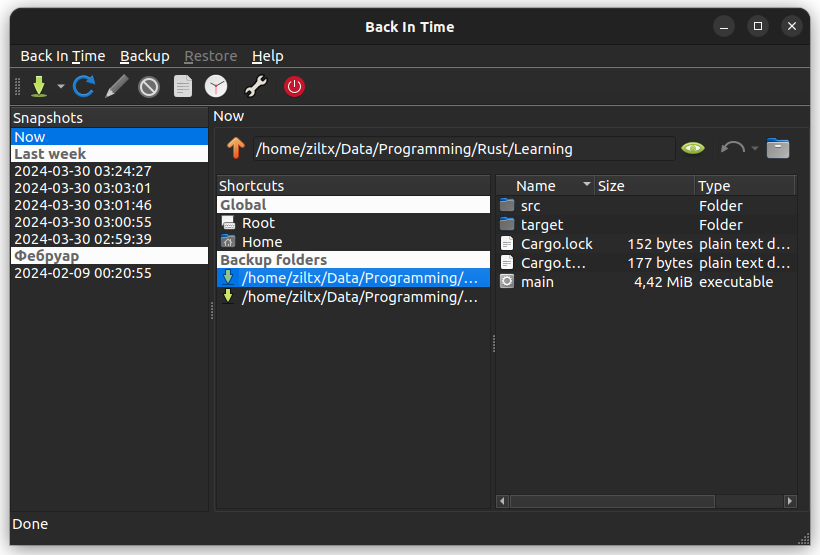
\includegraphics[width=0.8\textwidth]{figures/BackInTime}
    }
\end{frame}

\begin{frame}{pgBackRest}
    \textbf{pgBackRest}
    \begin{itemize}
        \item Supports full, incremental, and differential backups.
        \item Uses parallelism for faster operations.
        \item Supports cloud storage.
    \end{itemize}
\end{frame}

\begin{frame}{pgBackRest}
    \centering
    \includegraphics[width=0.7\textwidth]{figures/pgbackrest}
\end{frame}

\begin{frame}{Barman}
    \begin{itemize}
        \item Used for remote backups.
        \item Provides incremental backup and deduplication.
        \item Maintains a backup catalog.
    \end{itemize}
\end{frame}

\begin{frame}{Barman}
    \centering
    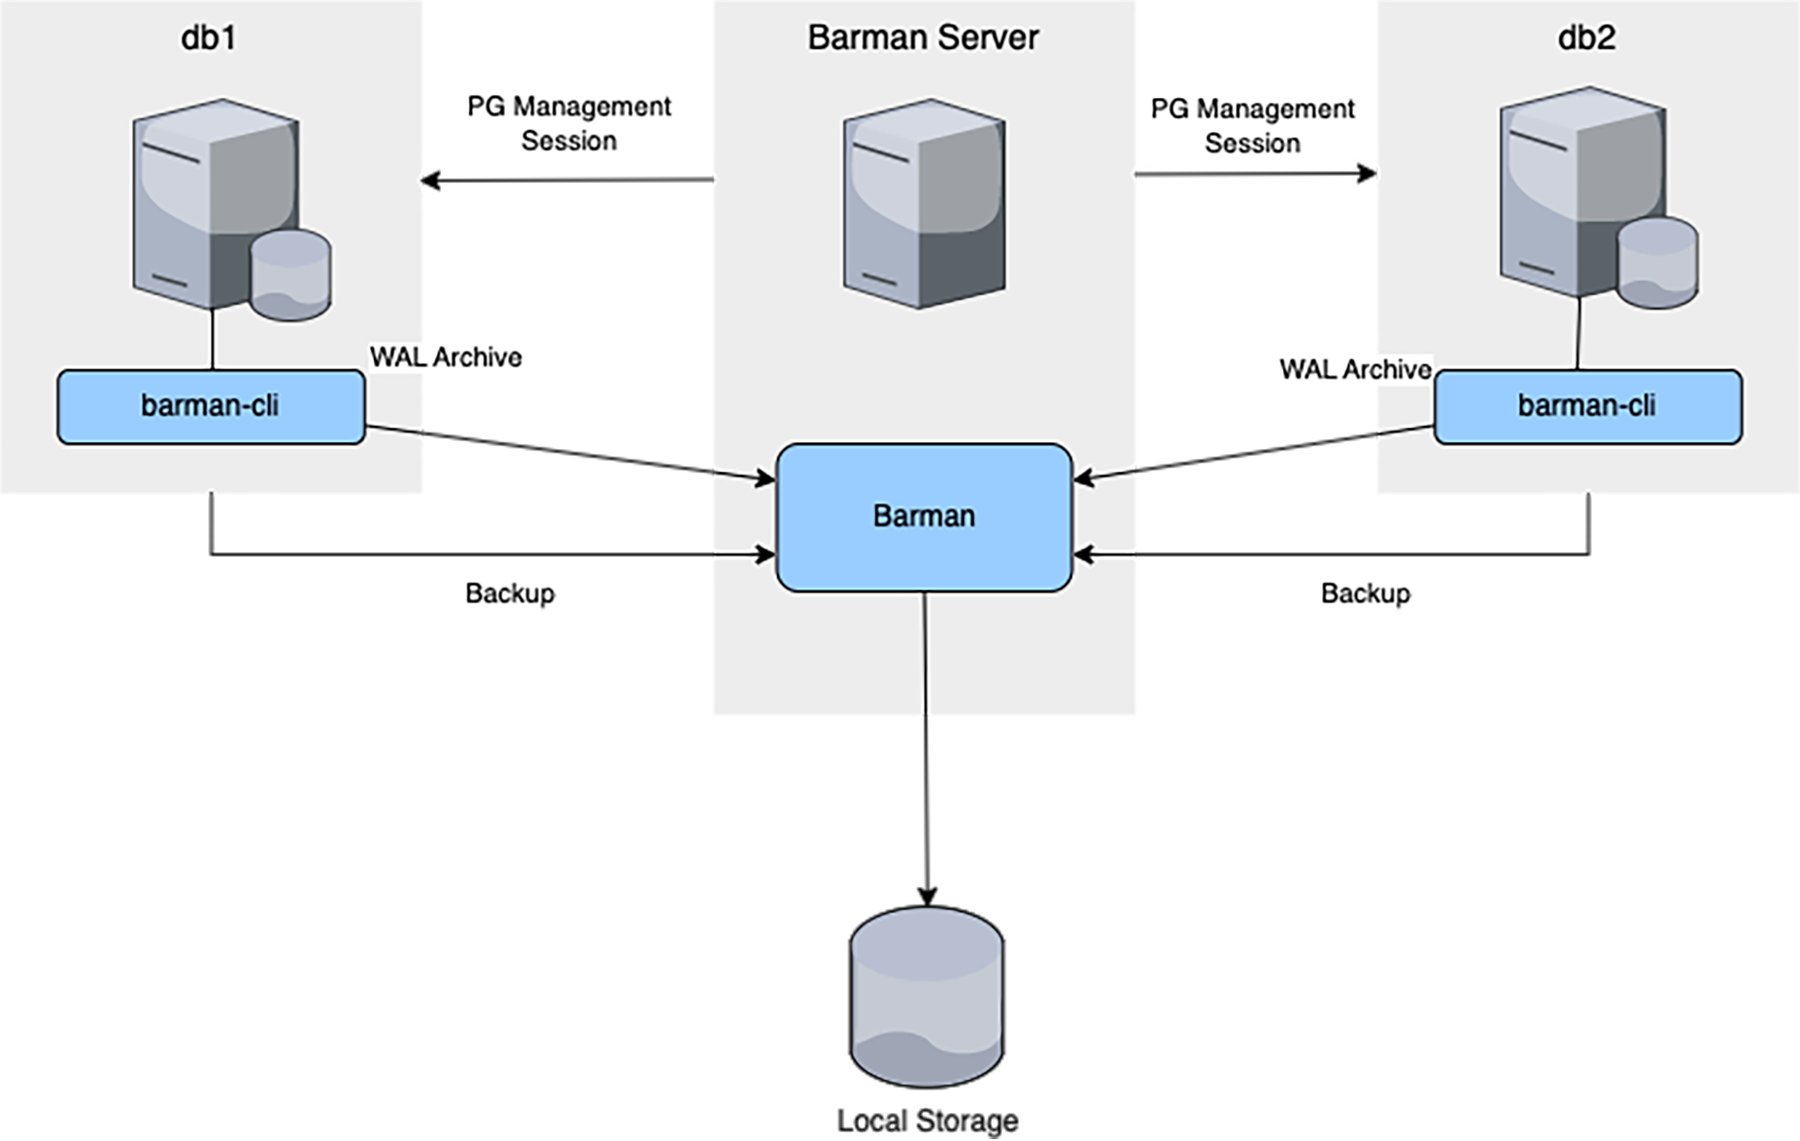
\includegraphics[width=0.7\textwidth]{figures/barman}
\end{frame}

\begin{frame}{pg\_probackup}
    \begin{itemize}
        \item Provides incremental restore to save time.
        \item Supports backup merging and deduplication.
        \item Offers parallelism and remote operations.
    \end{itemize}
\end{frame}

\begin{frame}{pg\_probackup}
    \centering
    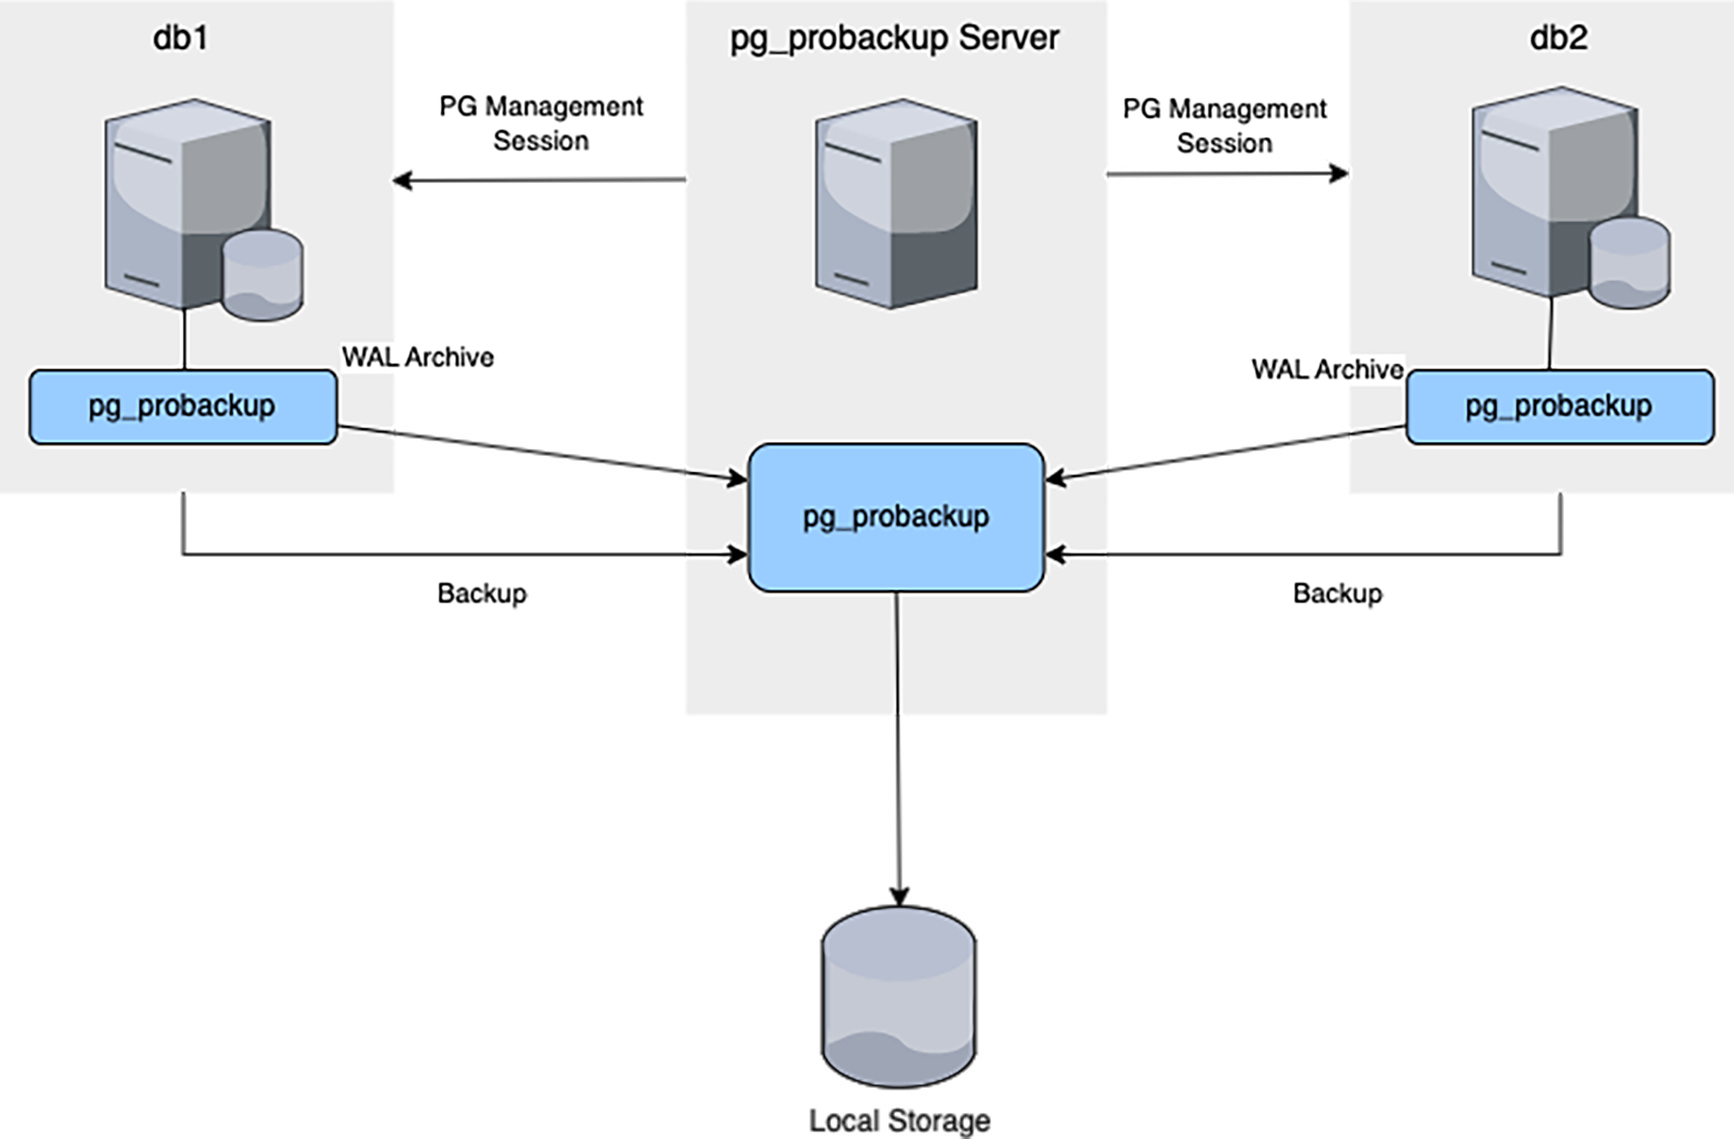
\includegraphics[width=0.7\textwidth]{figures/pg_probackup}
\end{frame}

\section*{Takeaways}

% Tim Duncan's Top 5 Fundamental Takeaways of the Today's Class
\begin{frame}{TDT5FTOTC}
    \centering
    
\includegraphics[height=0.9\textheight]{figures/tim.png}
\end{frame}

\begin{frame}{TDT5FTOTC}
    \pause
    \begin{itemize}
        \item[5] \textbf{Regular backups} are essential for ensuring high availability, enabling point-in-time recovery, and recovering from accidental changes. \pause

        \item[4] PostgreSQL supports \textbf{two main backup types}: physical (cluster-level, filesystem copy) and logical (human-readable, object-level, portable). \pause

        \item[3] \textbf{Built-in tools} like pg\_dump, pg\_dumpall, pg\_basebackup, psql, and pg\_restore allow creating and restoring different types of backups. \pause

        \item[2] \textbf{Point-in-Time Recovery} (PITR) requires WAL archiving and is only supported with physical backups, not logical ones. \pause

        \item[1] \textbf{Community tools} such as pgBackRest, Barman, and pg\_probackup provide advanced features like incremental backups, compression, cloud storage, and catalogs.
    \end{itemize}
\end{frame}

\begin{frame}{Database Administration: Backup and Restore.}
    \centering
    
\includegraphics[width=0.35\textwidth]{figures/book_cover}\\
    \vspace{2mm}
    {
        \scriptsize
        Content has been extracted from \textit{PostgreSQL for Jobseekers (Chapter 7)}, by Sonia Valeja and David Gonzales, 2023.  Visit \url{https://bpbonline.com/products/postgresql-for-jobseekers}.\\
    }
\end{frame}

\end{document}
